\section{Architecture and Software Design}
\label{sec:architecture}

Architecturally, the software product is comprised of three components. As shown on the schematic overview of the deployment (Fig~\ref{img:ksa-schematic-overview}), these components use HTTP API requests and Websockets for the communication. We can safely use unprotected HTTP protocol without TLS as the components are deployed inside one namespace and use internal communication channels only. We use websockets to notify frontend of events on the backend, which makes frontend very responsive, but tightly couples these components. A message queuing system like Kafka or RabbitMQ was considered as an alternative solution that would loosen the components and make them less dependant on each other, but it was decided against it as the system is not very big and messaging does not occur too often. Using message broker would only add extra complexity to the solution in our case.

From the feature perspective, the tool was designed to help DevSecOps engineer manage Kubernetes secuirty and, thus, serves the following requirements:
\begin{itemize}[noitemsep]
    \item User must be able to trigger the scan from the dashboard.
    \item Scanning and parsing should occur automatically without user interaction.
    \item Scan results should be persisted in the database for the future use.
    \item User must be able to browse the scan results.
    \item User must be able to search through the results.
    \item User must be able to generate reports based on the scan results.
    \item User must be able to manipulate findings (delete or mark as resolved).
    \item Dashboard should provide the possibility to be extended with other security scanners in the future.
    \item Dashboard should be able to generate graphic visualisation of the scan results.
\end{itemize}

The component diagram on the Fig~\ref{img:ksa-component-diagram} illustrates the architecture of a Kubernetes-native security scanning system. The process begins with the Dashboard component, which allows users to trigger scans and query results. Scan requests are forwarded to the Aggregator, which continues the process by initiating and watching for the scan job through the Kubernetes API. The Kubernetes API is responsible for scheduling the execution of containerized scanner jobs (such as Trivy, Kube-bench, and Prowler) within the cluster. Once the scanners complete their tasks, Aggregator component initiates parsing by sending a request to the Parser component, results are then stored in the Database component, which supports query operations for both the Dashboard and Aggregator. Additionally, the Parser exposes a WebSocket endpoint that enables real-time updates to the Dashboard—notifying it asynchronously when scan results are available. This decoupled, event-driven approach improves system responsiveness and user experience.

\begin{figure}[!hbt]
	\begin{center}
		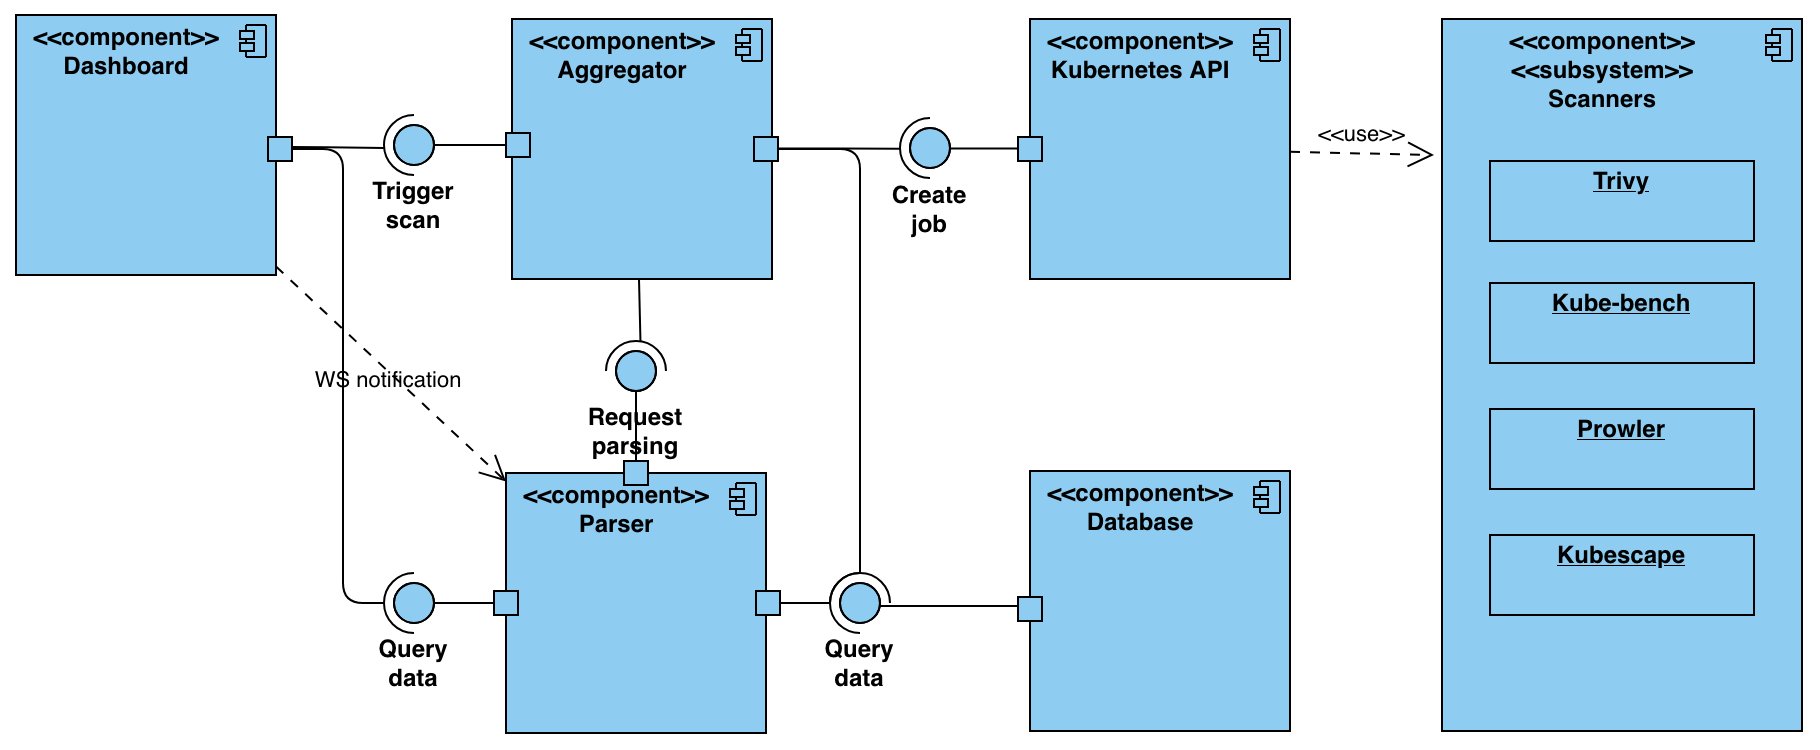
\includegraphics[width=0.9\textwidth]{images/ksa-component-diagram.png}
        \caption{Component diagram of the dashboard.}
		\label{img:ksa-component-diagram}
	\end{center}
\end{figure}

As seen on the Fig~\ref{img:ksa-schematic-overview}, both Parser and scanner Jobs mount the same PVC, where the results of the scan are stored. Each scanner has its own PersistentVolumeClaim, so that they can perform simultaneous writing uninterrupted. Those PVCs are mounted into specific directories on the Parser pod, that reads reports created by the scan jobs from these directories.

\begin{figure}[!hbt]
	\begin{center}
		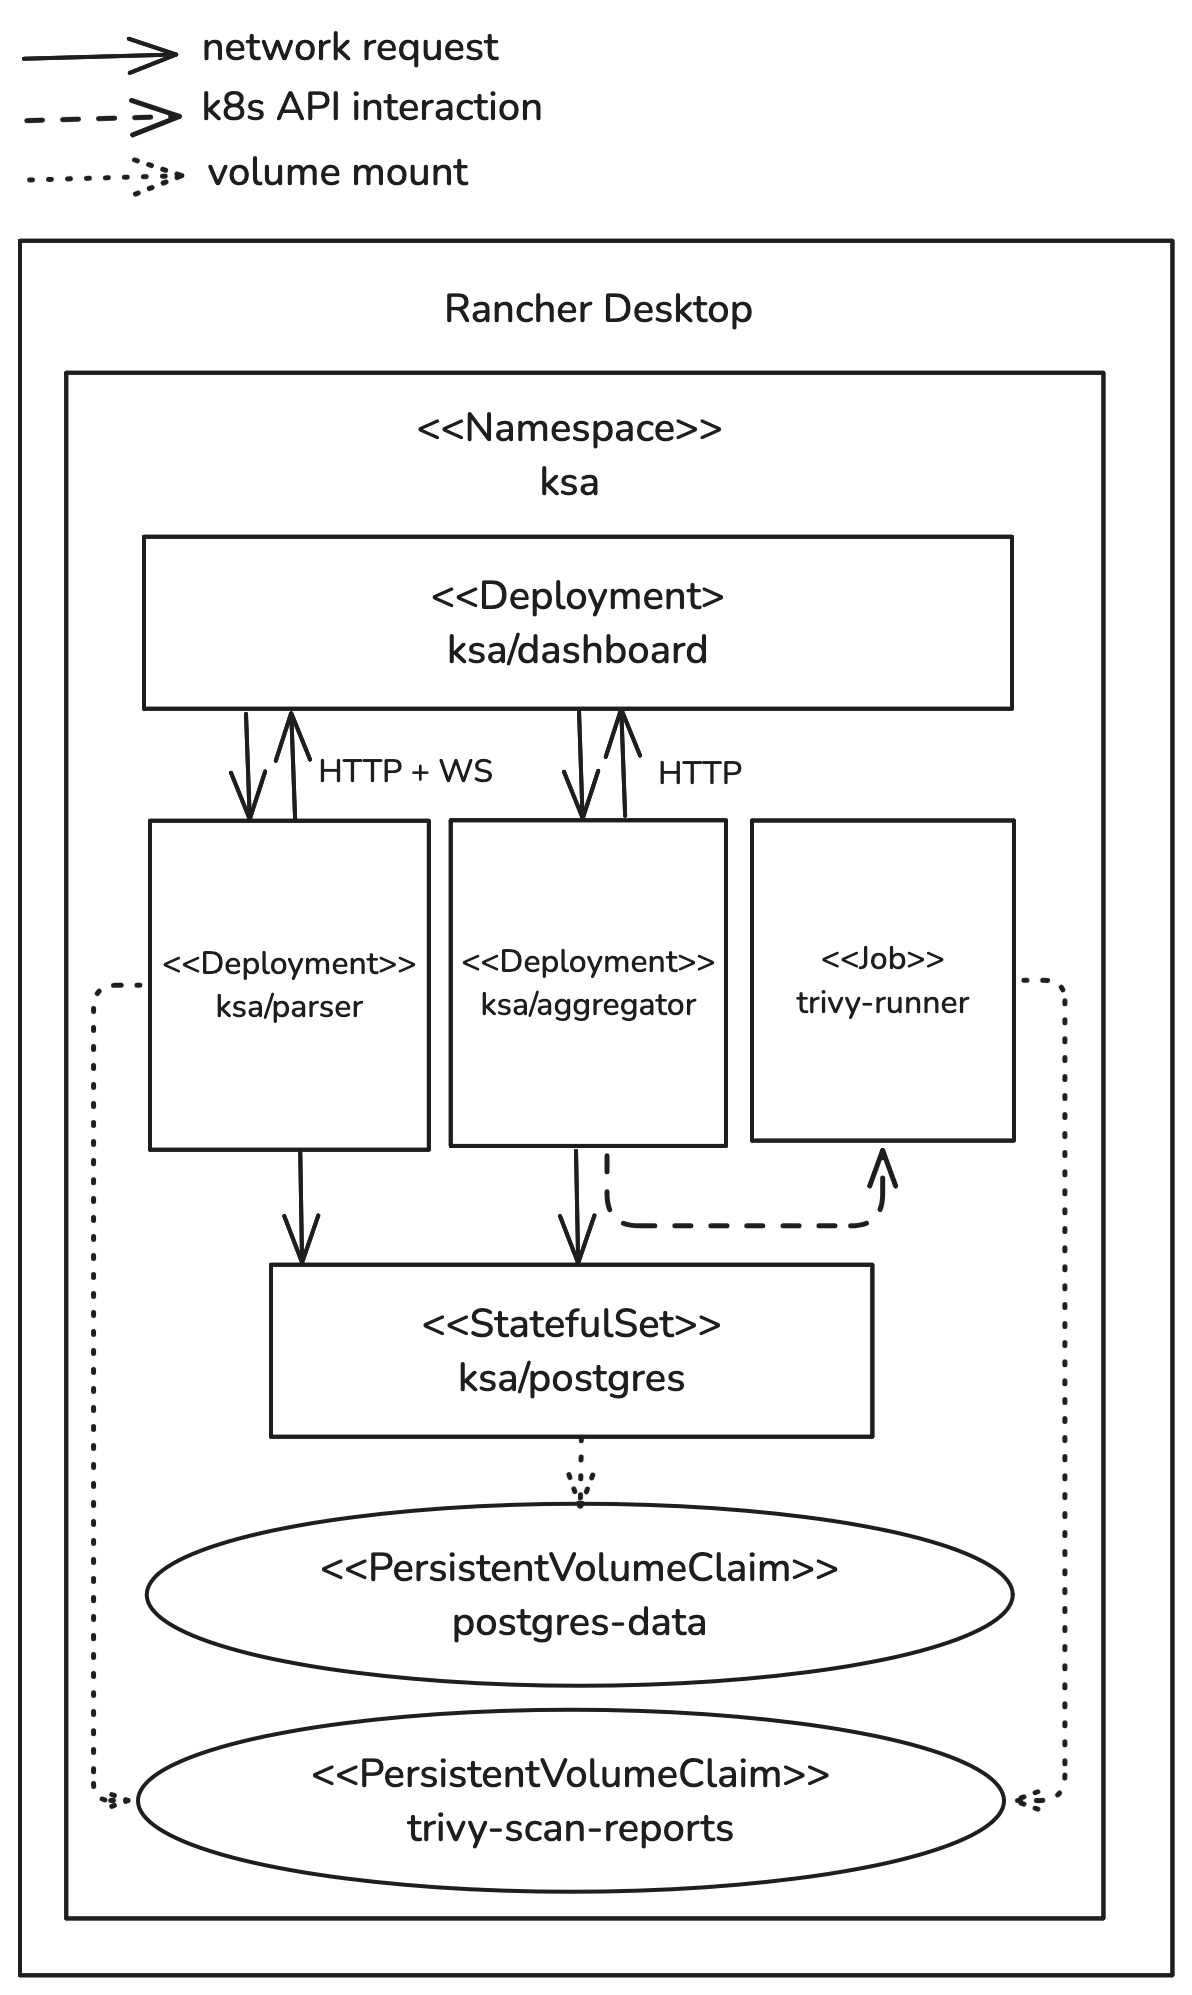
\includegraphics[width=0.5\textwidth]{images/ksa-schematic.png}
        \caption{A schematic overview of the KSA dashboard deployment.}
		\label{img:ksa-schematic-overview}
	\end{center}
\end{figure}